\begin{itemize}
	\item \textbf{Specification:} [NIST SP 800-38D] \\
	\url{https://csrc.nist.gov/pubs/sp/800/38/d/final}
	\item \textbf{Implementation:} \\
	\url{https://github.com/openssl/openssl/blob/master/crypto/modes/gcm128.c}
\end{itemize}
%\paragraph{References:} 
%\cite{McGrewViega2004gcm}
\begin{figure}[h!]\centering
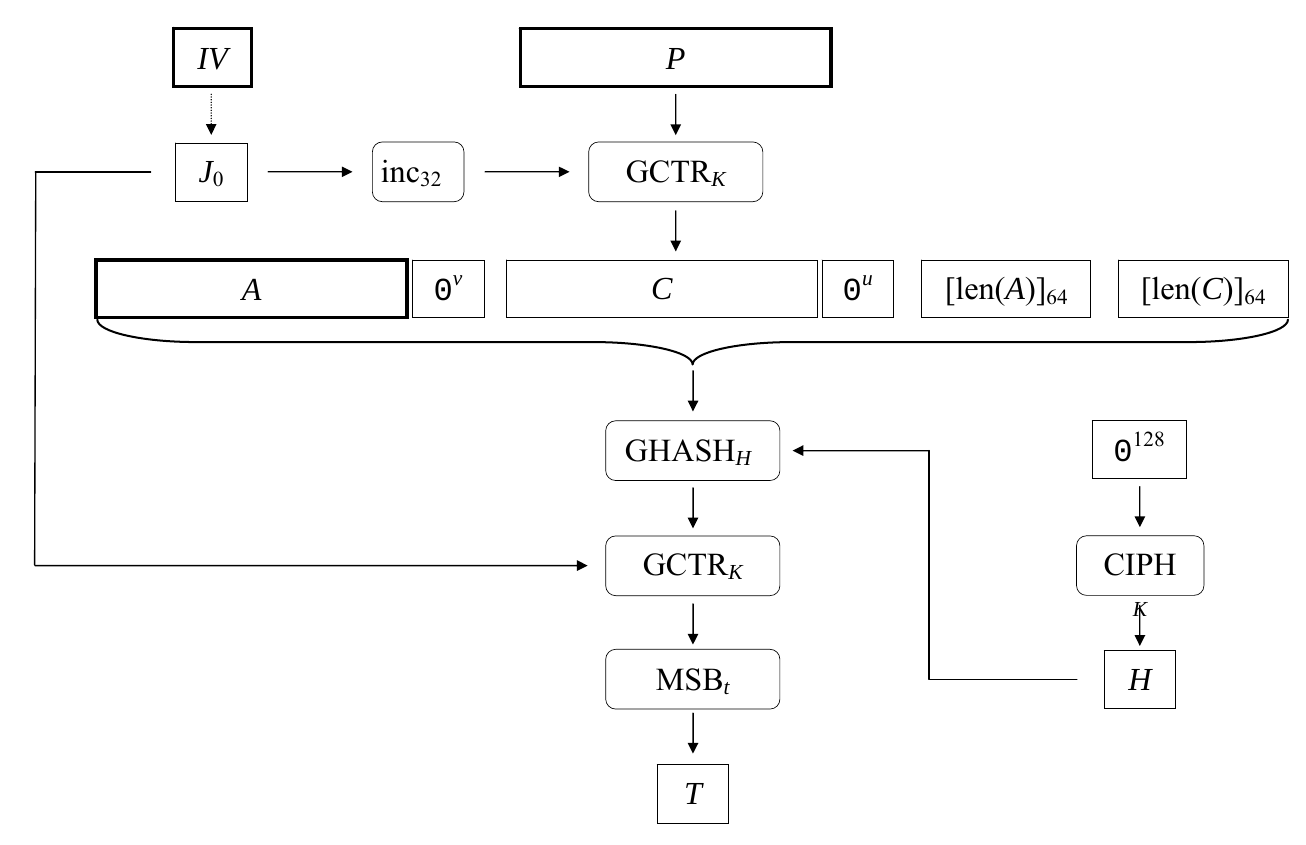
\includegraphics[scale=.325]{images/mode-gcm}
\caption{Illustration of ${\rm GCM}\text{-}{\rm AE}_K (IV, P, A) = (C, T)$ in NIST SP 800-38D (p16).}
\end{figure}

%------------------------------------------------------------
\begin{algorithm}[H]
	\caption{GCM Authenticated Encryption ${\rm GCM\text{-}AE}_K(IV,P,A)$}\label{alg:gcm-ae}
	\KwIn{\begin{itemize}
			\item 
		\end{itemize}Key $K$, IV, Plaintext $P$, AAD $A$, tag‐length $t$}
	\KwOut{Ciphertext $C$, Authentication Tag $T$}
	% prerequisites
	$H \gets \mathrm{CIPH}_K(\texttt{0}^{128})$\;
	\uIf{$|\,\mathrm{IV}\,| = 96$}{
		$J_0 \gets \mathrm{IV}\,\|\,0^{31}\,\|\,1$\;
	}\Else{
		$s \gets 128\cdot\bigl\lceil|\,\mathrm{IV}\,|/128\bigr\rceil - |\,\mathrm{IV}\,|$\;
		$J_0 \gets \mathrm{GHASH}_H\bigl(\mathrm{IV}\,\|\,0^s\,\|\,[\!|\,\mathrm{IV}\,|\!]_{64}\bigr)$\;
	}
	$C \gets \mathrm{GCTR}_K\bigl(\mathrm{inc}_{32}(J_0),\,P\bigr)$\;
	\BlankLine
	$v \gets 128\cdot\lceil|A|/128\rceil - |A|$\;
	$u \gets128\cdot\lceil|C|/128\rceil - |C|$\;
	$S \gets \mathrm{GHASH}_H\bigl(A\,\|\,0^v\,\|\,C\,\|\,0^u\,\|\,[\!|A|\!]_{64}\,\|\,[\!|C|\!]_{64}\bigr)$\;
	$T \gets \mathrm{MSB}_t\bigl(\mathrm{GCTR}_K(J_0,\,S)\bigr)$\;
	\Return{$(C,T)$}\;
\end{algorithm}

%------------------------------------------------------------
\begin{algorithm}[H]
\caption{GCM Authenticated Decryption (GCM-AD\_K)}\label{alg:gcm-ad}
\KwIn{Key $K$, IV, Ciphertext $C$, AAD $A$, Tag $T$, tag‐length $t$}
\KwOut{Plaintext $P$ or \textsf{FAIL}}
\If{$|T|\neq t$ \textbf{or} lengths not supported}{%
	\Return{\textsf{FAIL}}%
}
$H \gets \mathrm{CIPH}_K(0^{128})$\;
\uIf{$|\,\mathrm{IV}\,| = 96$}{
	$J_0 \gets \mathrm{IV}\,\|\,0^{31}\,\|\,1$\;
}
\Else{
	$s \gets 128\cdot\bigl\lceil|\,\mathrm{IV}\,|/128\bigr\rceil - |\,\mathrm{IV}\,|$\;
	$J_0 \gets \mathrm{GHASH}_H\bigl(\mathrm{IV}\,\|\,0^s\,\|\,[\!|\,\mathrm{IV}\,|\!]_{64}\bigr)$\;
}
$P \gets \mathrm{GCTR}_K\bigl(\mathrm{inc}_{32}(J_0),\,C\bigr)$\;
\BlankLine
$v \gets 128\cdot\lceil|A|/128\rceil - |A|$\;\quad
$u \gets128\cdot\lceil|C|/128\rceil - |C|$\;
$S \gets \mathrm{GHASH}_H\bigl(A\,\|\,0^v\,\|\,C\,\|\,0^u\,\|\,[\!|A|\!]_{64}\,\|\,[\!|C|\!]_{64}\bigr)$\;
$T' \gets \mathrm{MSB}_t\bigl(\mathrm{GCTR}_K(J_0,\,S)\bigr)$\;
\If{$T' = T$}{
	\Return{$P$}\;
}
\Else{
	\Return{\textsf{FAIL}}\;
}
\end{algorithm}

\newpage
\subsection{Data Structure}
\begin{lstlisting}[style=cstyle]
#if defined(__x86_64) || defined(__x86_64__)
#	define BSWAP8(x) ({ u64 ret_=(x); \
						asm ("bswapq %0"\
						: "+r"(ret_)); ret_; })
#   define BSWAP4(x) ({ u32 ret_=(x); \
						asm ("bswapl %0" \
						: "+r"(ret_));   ret_; })
#endif

#if defined(BSWAP4) && !defined(STRICT_ALIGNMENT)
# define GETU32(p)       BSWAP4(*(const u32 *)(p))
# define PUTU32(p,v)     *(u32 *)(p) = BSWAP4(v)
#else
# define GETU32(p)       ((u32)(p)[0]<<24|(u32)(p)[1]<<16|(u32)(p)[2]<<8|(u32)(p)[3])
# define PUTU32(p,v)     ((p)[0]=(u8)((v)>>24),(p)[1]=(u8)((v)>>16),(p)[2]=(u8)((v)>>8),(p)[3]=(u8)(v))
#endif

/*- GCM definitions */ typedef struct {
	u64 hi, lo;
} u128;


typedef void (*gcm_init_fn)(u128 Htable[16], const u64 H[2]);
typedef void (*gcm_ghash_fn)(u64 Xi[2], const u128 Htable[16], const u8 *inp, size_t len);
typedef void (*gcm_gmult_fn)(u64 Xi[2], const u128 Htable[16]);
struct gcm_funcs_st {
	gcm_init_fn ginit;
	gcm_ghash_fn ghash;
	gcm_gmult_fn gmult;
};	
	
struct gcm128_context {
	/* Following 6 names follow names in GCM specification */
	union {
		u64 u[2];
		u32 d[4];
		u8 c[16];
		size_t t[16 / sizeof(size_t)];
	} Yi, EKi, EK0, len, Xi, H;
	/*
	* Relative position of Yi, EKi, EK0, len, Xi, H and pre-computed Htable is
	* used in some assembler modules, i.e. don't change the order!
	*/
	u128 Htable[16];
	struct gcm_funcs_st funcs;
	unsigned int mres, ares;
	block128_f block;
	void *key;
};
\end{lstlisting}

\newpage
\subsection{title}







\iffalse
\subsection{Multiplication in $\GF(2^{128})$}
\begin{definition}
	Let \(\mathbb F_2 = \{0,1\}\) be the field with two elements.  Fix an irreducible polynomial
	\[
	f(x) \;=\; x^{128} + x^7 + x^2 + x + 1 
	\quad\in\; \mathbb F_2[x].
	\]
	Then
	\[
	\mathrm{GF}(2^{128}) \;=\; \mathbb F_2[x] \,\big/\,\bigl(f(x)\bigr)
	\]
	is the degree-\(128\) binary extension field.
\end{definition}
\begin{remark}
Every element \(\alpha\in\mathrm{GF}(2^{128})\) can be written uniquely as \[
\alpha \;=\; a_{127}x^{127} + a_{126}x^{126} + \cdots + a_1 x + a_0
\quad(a_i\in\{0,1\}).
\] We identify \(\alpha\) with the \(128\)-bit vector \((a_{0},\dots,a_{127})\in\F_2\).
\end{remark}

\paragraph{Polynomial Representation and Reduction}
Consider \[
\left(\sum_{i=0}^{127}a_i x^i\right)\,\left(\sum_{j=0}^{127}b_j x^j\right)
\;=\;\sum_{i=0}^{127}\sum_{j=0}^{127}(a_i b_j)\,x^{i+j},\quad\text{where each $a_i b_j\in\{0,1\}$}.
\] The raw product has degree at most 254.  To obtain an element of 
\(\GF(2^{128})\), we reduce it modulo $
f(x)=x^{128}+x^7+x^2+x+1$.
Concretely, whenever a term \(x^k\) with \(k\ge128\) appears, one replaces 
\[
x^{128}\;\mapsto\;x^7+x^2+x+1
\]
and iterates until the remainder has degree \(\le127\).

\paragraph{Bit-Level Algorithm}
We implement multiplication by a simple ``shift-and-add'' method with reduction on each
shift, often called \(\mathtt{gf128\_xtime}\). For \(v\in\mathrm{GF}(2^{128})\) represented as a 128-bit, define a function \[
\texttt{gf128\_xtime}:\GF(2^{128})\to\GF(2^{128}),\quad v\mapsto xv.
%\fullfunction{\texttt{gf128\_xtime}}{\GF(2^{128})}{\GF(2^{128})}{v}{x\cdot v}.
\] for each $v\in\GF(2^{128})$. Since \begin{align*}
\texttt{gf128\_xtime}(v)=x\cdot v
%&=x\cdot(a_{127}a_{126}\cdots a_{120}\parallel\cdots\parallel a_{14}a_{13}\cdots a_{8}\parallel a_7a_6\cdots a_0) \\
%&=x\cdot (a_{127}x^{127}+a_{126}x^{126}+\cdots a_2x^2+a_1x+a_0) \\
%&=a_{127}{\color{red}x^{128}}+a_{126}x^{127}+\cdots a_2x^3+a_1x^2+a_0x \\
%&=a_{127}{\color{red}(1+x+x^2+x^7)}+a_{126}x^{127}+\cdots a_2x^3+a_1x^2+a_0x \\
%&=\begin{cases*}
%	a_{126}\cdots a_{119}\parallel\cdots\parallel a_{14}\cdots a_{7}\parallel (a_6\cdots a_00\oplus\;\texttt{00000000})\parallel   &if $a_{127}=0$\\
%	a_{126}\cdots a_{119}\parallel\cdots\parallel a_{14}\cdots a_{7}\parallel (a_6\cdots a_00\oplus\;\texttt{10000111})\parallel   &if $a_{127}=1$
%\end{cases*},
&=x\cdot(a_{0}a_{1}\cdots a_{7}\parallel a_{8}a_{9}\cdots a_{15}\parallel\cdots\parallel a_{120}a_{121}\cdots a_{127}) \\
&=x\cdot (a_0+a_1x+\cdots +a_{126}x^{126} +a_{127}x^{127}) \\
&=a_0x+a_1x^2+\cdots+a_{126}x^{127}+a_{127}{\color{red}x^{128}}\\
&=a_0x+a_1x^2+\cdots+a_{126}x^{127}+a_{127}{\color{red}(x^7+x^2+x+1)}\\
&=\begin{cases*}
(0a_1\cdots a_6\oplus\;\texttt{00000000})\parallel a_{7}\cdots a_{14}\parallel\cdots\parallel a_{119}a_{120}\cdots a_{126}  &if $a_{127}=0$\\
(0a_1\cdots a_6\oplus\;\texttt{11100001})\parallel a_{7}\cdots a_{14}\parallel\cdots\parallel a_{119}a_{120}\cdots a_{126}  &if $a_{127}=1$
\end{cases*},
\end{align*} we have
\[
\mathtt{gf128\_xtime}(v) = 
\begin{cases}
	v \gg 1, &\text{if the MSB of }v\text{ is }0,\\[6pt]
	(v \gg 1)\oplus\texttt{0xE1}, &\text{if the MSB of }v\text{ is }1,
\end{cases}
\]
where \texttt{0xE1} is the bit-vector corresponding to the reduction polynomial
\(x^7+x^2+x+1\).
\vfill
\begin{lstlisting}[style=cstyle]
/* v <- vx mod (x^128 + x^7 + x^2 + x + 1) */
void gf128_xtime(uint8_t v[16]) {
	uint8_t t = v[15] & 1;				// p[15] = p120...p127; extract p127
	// Shift the 128-bit value right by 1:
	for (int i = 15; i > 0; --i)		
		v[i] = (v[i] >> 1) | ((v[i-1] & 1) << 7);
	p[0] >>= 1;							// p0p1...p7 -> 0p0...p6
	if (t) v[0] ^= 0xE1;                // // 0p0...p6 ^ 11100001
}
\end{lstlisting}

%* Inputs & outputs are 128-bit values in big-endian byte order (p[0]...p[15]).
\begin{lstlisting}[style=cstyle]
/*
* Compute p(x) <- p(x)q(x) over GF(2^128) using "shift-and-add" multiplication.
*/
void gf128_mul(u8 p[16], u8 q[16]) {
	u8 buffer[16] = { 0x00, };      // accumulator for the product
	u8 bit_mask;              // mask for each bit of q
	for (int i = 0; i < 16; ++i) { // Loop over each byte of q (Q[0] = q120...q127)
		for (int j = 0; j < 8; ++j) { // Process bits q(128-8i-1) down to q(128-8i-8)
			bit_mask = q[i] & (1 << (7 - j));
			if (bit_mask) {
				// If the current bit of q is 1, XOR the current p(x) into buffer
				for (int k = 0; k < 16; ++k) { buffer[k] ^= p[k]; }
			}
			gf128_xtime(p); // Multiply p(x) by x (i.e. shift-and-reduce) for next bit
		}
	}
	// Write the accumulated product back into p[0...15]
	for (int i = 0; i < 16; ++i) { p[i] = buffer[i]; }
}
\end{lstlisting}
\newpage

\subsection{Efficient Multiplication in $\GF(2^{128})$}
TBA
%\paragraph{Pseudocode}
%\ \\ \begin{algorithm}[H]
%	\caption{Multiply two field elements \(a,b\in\mathrm{GF}(2^{128})\)}
%	\label{alg:mul2}
%	\begin{algorithmic}[1]
%		\REQUIRE \(a,b\in\{0,1\}^{128}\) as 128-bit words  
%		\ENSURE \(c = a\cdot b \bmod f(x)=x^{128}+x^7+x^2+x+1\)
%		\STATE \(c \leftarrow 0\)  
%		\STATE \(v \leftarrow a\)  
%		\FOR{\(i=0\) to \(127\)}  
%		\IF{bit \(i\) of \(b\) is 1}  
%		\STATE \(c \leftarrow c \oplus v\)  
%		\ENDIF  
%		\STATE \(v \leftarrow \mathtt{xtime}(v)\)  
%		\ENDFOR  
%		\RETURN \(c\)
%	\end{algorithmic}
%\end{algorithm}
\fi